\usetheme{metropolis}

\usepackage{appendixnumberbeamer}

\usepackage{booktabs}
\usepackage[scale=2]{ccicons}

\usepackage{pgfplots}
\usepgfplotslibrary{dateplot}

\usepackage{xspace}
\newcommand{\themename}{\textbf{\textsc{metropolis}}\xspace}

\metroset{titleformat frame=smallcaps}

% Add section numbers in TOC
% https://tex.stackexchange.com/a/44998/173708
\setbeamertemplate{section in toc}[sections numbered]

%%% Local Variables:
%%% mode: latex
%%% TeX-master: t
%%% End:


% make background color for title of the slides green
% https://tex.stackexchange.com/a/360349/173708
\definecolor{OilGainsGreen}{RGB}{85, 130, 5}    % Fidelity green normal
\definecolor{OilGainsGreenDark}{RGB}{65, 95, 5}    % Fidelity dark
\definecolor{OilGainsNight}{RGB}{55, 85, 5}        % Fidelity darker
\setbeamercolor{frametitle}{bg=OilGainsGreenDark}   % do not change foreground color


% set folder for figures
\graphicspath{{figs/}}


% % remove the [rt] keyword. Offset and increase to maximum size
% % https://tex.stackexchange.com/a/412707/173708
% \titlegraphic{%
%   \begin{picture}(0,0)
%     \put(154,-114){\makebox(0,0){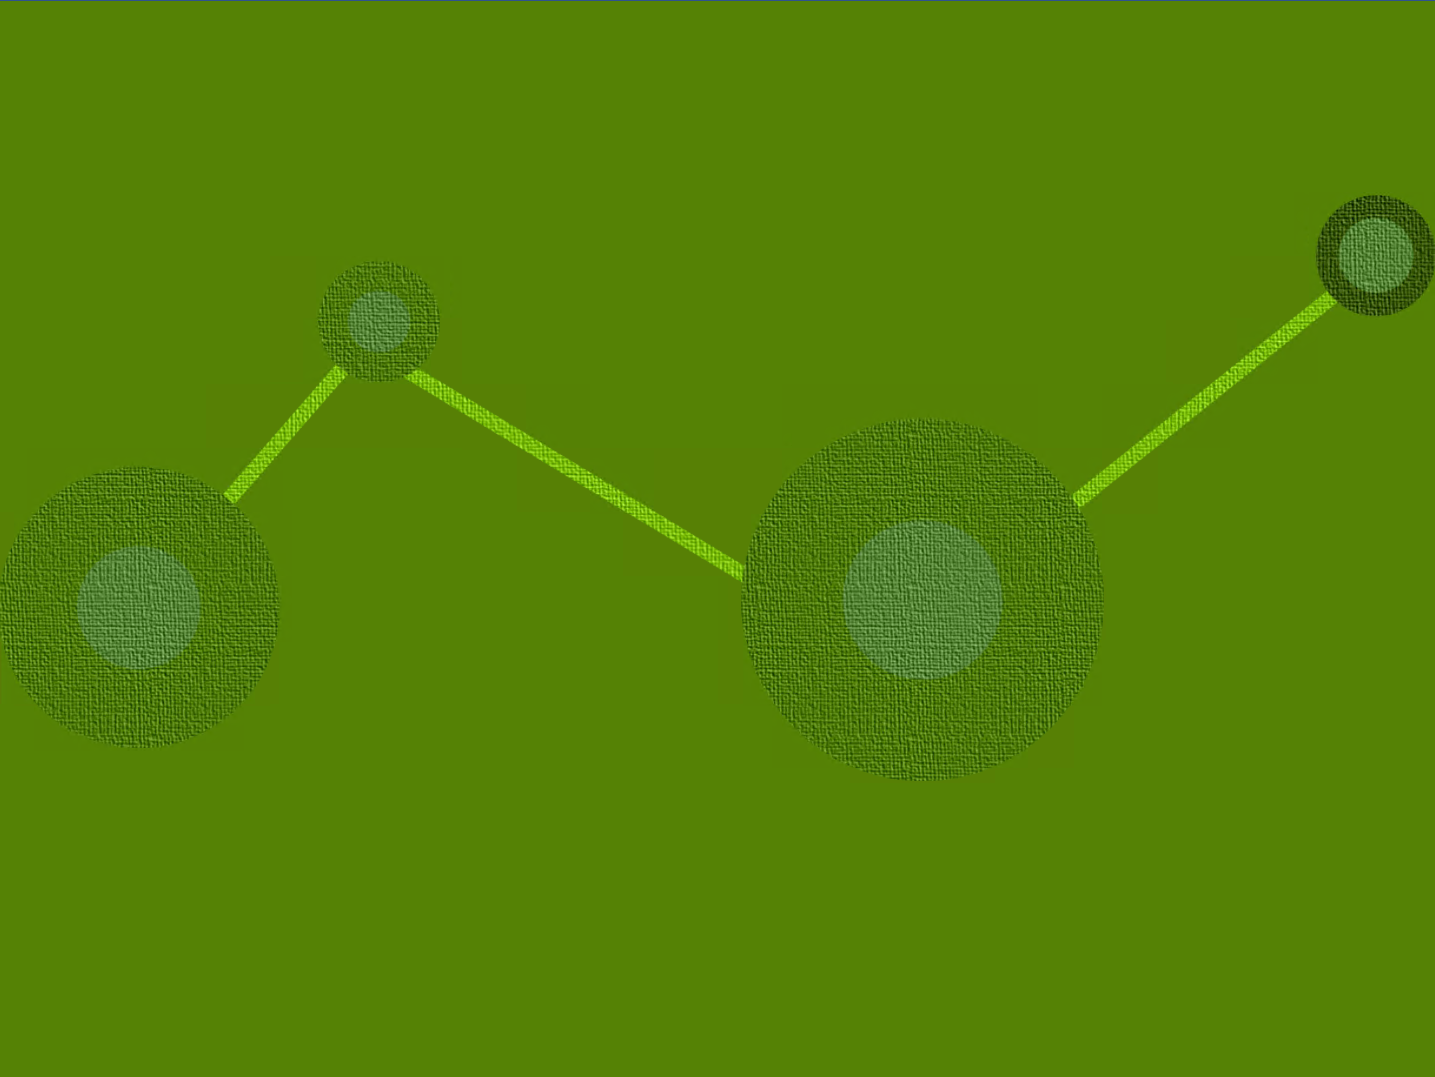
\includegraphics[width=\paperwidth,height=\paperheight]{OilGainsTitleSlide2}}}
%   \end{picture}}


% % change color of title and subtitle
\definecolor{OilGainsGreen}{RGB}{85, 130, 5}  % Fidelity green normal
% \setbeamercolor{title}{fg=white,bg=OilGainsGreen}
% \setbeamercolor{subtitle}{fg=yellow,bg=OilGainsGreen}
% \setbeamercolor{author}{fg=white,bg=OilGainsGreen}
% \setbeamercolor{date}{fg=white,bg=OilGainsGreen}
% \setbeamercolor{institute}{fg=yellow,bg=OilGainsGreen}

% % change color of the progress bar and title separator
% \definecolor{blueucl}{RGB}{0,87,156} %which is the color of my university
% \setbeamercolor{progress bar}{fg=blueucl}
% \setbeamercolor{title separator}{fg=lightgray} % color of the title separator
% \setbeamercolor{progress bar in head/foot}{fg=blueucl}
% \setbeamercolor{progress bar in section page}{fg=OilGainsGreen}


% change color standout slide
% https://github.com/matze/mtheme/issues/234
\definecolor{myGreen}{RGB}{30,98,56}
\definecolor{myGold}{RGB}{226,168,43}
% keep colors white and OilGainsGreen
\setbeamercolor{palette primary}{fg=white, bg=OilGainsGreenDark}

% change TOC color
% https://tex.stackexchange.com/a/29332/173708
\colorlet{mycolor}{orange!80!black}% change this color to suit your needs
\setbeamercolor{section in toc}{fg=mycolor}
\setbeamercolor{subsection in toc shaded}{fg=black}

% change thickness of progress bar and title separator
% https://github.com/matze/mtheme/issues/237
\makeatletter
\setlength{\metropolis@titleseparator@linewidth}{0.25pt}
\setlength{\metropolis@progressonsectionpage@linewidth}{2pt}
\setlength{\metropolis@progressinheadfoot@linewidth}{2pt}
\makeatother

% \logo{the logo \raisebox{0.5cm}{
\includegraphics[width=1cm]{logo}}\hspace*{\textwidth}}

% place the logo at the bottom of each slide
% https://tex.stackexchange.com/a/341702/173708
\usepackage{graphbox}
\setbeamertemplate{footline}{%
    
\includegraphics[align=c, height=0.45cm]{oilgains-alegr}%
    \hfill%
    \usebeamercolor[fg]{page number in head/foot}%
    \usebeamerfont{page number in head/foot}%
    \insertframenumber\,/\,\inserttotalframenumber\kern1em%
}
